% TEX compiler = latexmk
% copyright arturo salinas-aguayo 2024
\documentclass[12pt]{article}

\usepackage{graphicx}
\usepackage{amsmath}
\usepackage{array}
\usepackage{amsfonts}
\usepackage{fancyhdr}
\usepackage{geometry}
\usepackage{circuitikz}
\usepackage{subfigure}
\usepackage{caption}
\usepackage{karnaugh-map}
\usepackage{bm}
\usepackage[table]{xcolor}
\usepackage{float}
\usepackage{subcaption}

\geometry{letterpaper, margin=1in}
\graphicspath{ {../images/} }

% Header and Footer
\pagestyle{fancy}
\fancyhf{}
\fancyhead[L]{CSE 2301 - Lab 11: Programmable Logic Arrays}
\fancyhead[R]{\thepage}
\setlength{\headheight}{15pt}

\author{Arturo Salinas-Aguayo}
\title{Lab 11: Programmable Logic Arrays}
% theorem set
\newtheorem{example}{Example}
% Example block environment
\newenvironment{examp}
{
	\vspace{.5cm}
	\hrule
\begin{example}\upshape}
	{\hrule
		\vspace{0.5cm}
\end{example}}

\begin{document}
\newcommand{\closure}[2][3]{%
	{}\mkern#1mu\overline{\mkern-#1mu#2}}
\newcommand\ncoverline[1]{\mkern1mu\overline{\mkern-1mu#1\mkern-1mu}\mkern1mu}
% Title Page
\begin{titlepage}
	\centering
	\vspace*{3cm}
	\huge\textbf{Lab 11: Programmable Logic Arrays}\\
	\vspace{5cm}
	\Large\textbf{Arturo Salinas-Aguayo}\\
	\normalsize
	CSE 2301: Principles and Practice of Digital Logic Design\\
	Dr. Mohammad Khan, Section 003L-1248\\
	Electrical and Computer Engineering Department
	\vfill
	
\includegraphics[scale=0.1]{uconnlogo}\\
	College of Engineering, University of Connecticut\\
	\scriptsize{Coded in \LaTeX}
	\vspace*{1cm}
\end{titlepage}
\section*{Discussion}
This lab dives into describing and designing what Programmable Logic Arrays
consist of and how they are packaged. Firstly, the entire course has utilized
conventional simplification of boolean algebra utilizing the Quine-McClusky
and the Karnaugh Map methods as well as the standard Boolean Algebra
simplification methods.

However, this lab marks a transition from theoretical simplification to practical implementation, giving students a glimpse of how real-world engineers approach circuit design. In practice, engineers move beyond discrete logic chips like the 7400 series and simple hand-drawn logic gate configurations. Instead, they rely on sophisticated Computer-Aided Design (CAD) tools that integrate Hardware Description Languages (HDLs) such as VHDL or Verilog.

These tools streamline the design process by offering automated \textit{place and route} capabilities. This allows designers to focus on high-level functionality, with software handling optimization for the targeted hardware.
\begin{examp}
\vspace{.5mm}
\textbf{Karnaugh-Map Review}\\
This exercise required a 5 Variable Karnaugh-Map, merely to show how much effort
it takes to traditionally solve these simplification questions compared to the
upcoming simplicity of the PLA.

\begin{center}
\begin{karnaugh-map}(label=corner)[4][4][2][$B$][$A$][$C_0$][$C_1$][$C_2$]
\minterms{0,1,2,3,5,6,7,8,9,10,13,14,16,19,23,24}
\implicant{1}{9}
\implicant{2}{10}
\implicant{3}{7}[0,1]
\implicantedge{0}{0}{8}{8}[0,1]
\autoterms[0]
\end{karnaugh-map}
\end{center}
\[
	F = \closure{C_0}\closure{A}\closure{B} + \closure{C_1}AB +
	\closure{C_2}\closure{A}B + \closure{C_2}A\closure{B}
\]
With the PLA implementation, each minterm for each output bit is placed and
routed by the software and abstracted away from the wires. For the \(C_2 = 0\)
block, notice how there are potential hazards at bay. These are kept separate in
order to best maximize the effect of the 3-Dimensional 5 Variable Karnaugh Map.
In this case, the blue and yellow squares ``wrap around" the corresponding
\(C_2\) block.
\begin{figure}[H]
	\center{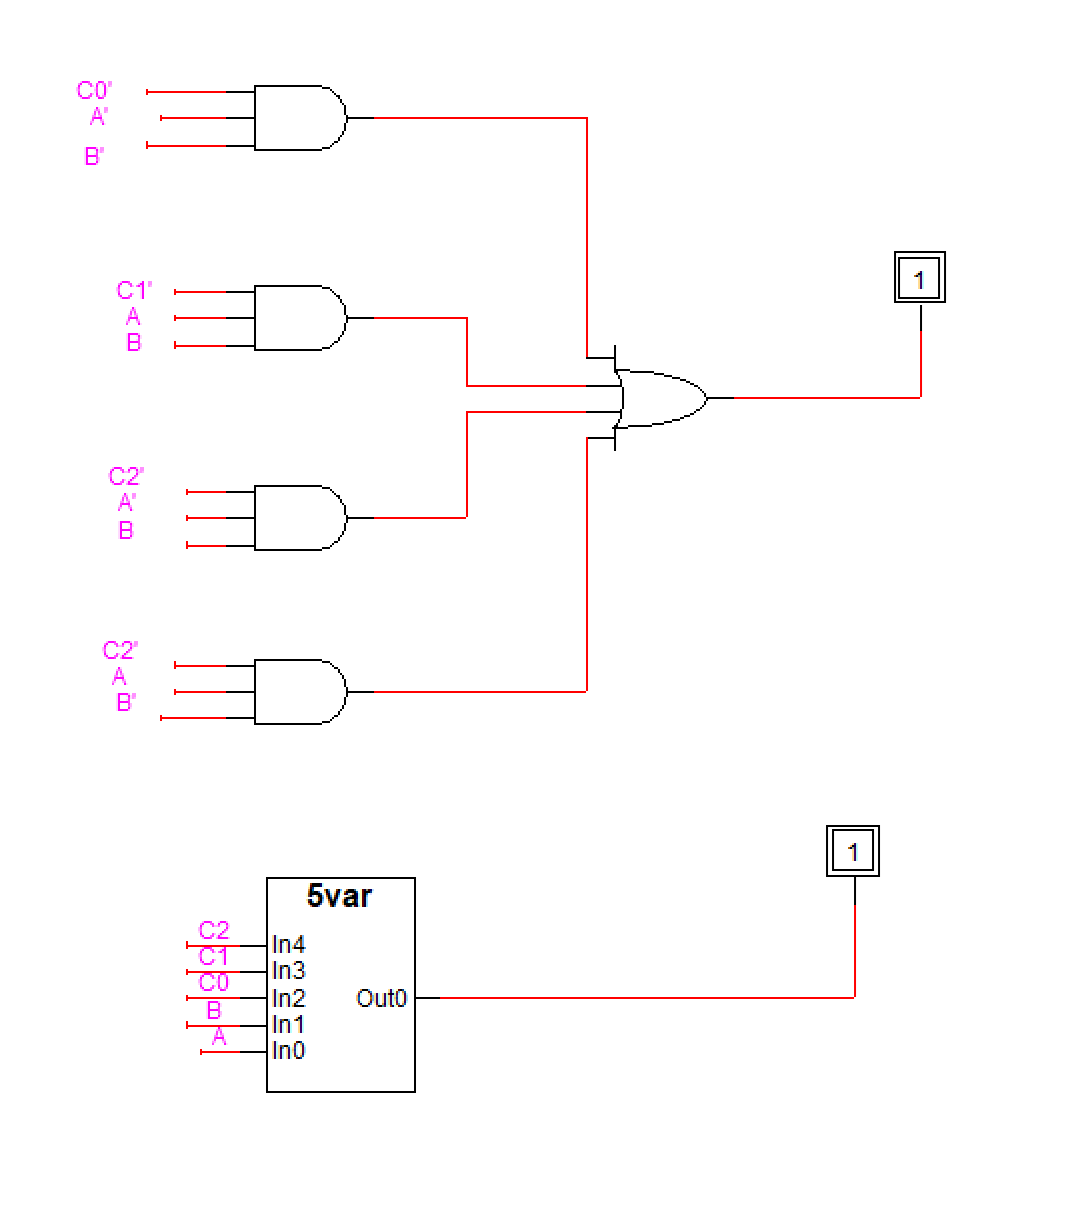
\includegraphics[scale=.60]{examp113}}
	\caption{Traditional Gate Implementation and Black Box
		Implementation}
\end{figure}
The PLA form greatly reduces the complexity of visual schematic design by
abstracting away the gate logic by programming it directly.
\end{examp}

\begin{examp}
	\vspace{.5mm}
	\textbf{A Continuation of the Triangle Parity}

	In this lab, we examined a 15-bit data stream configured with EVEN parity using a triangular code. The output identifies error positions by mapping the detected location to a four-bit decimal representation. An error is flagged whenever a mismatch in parity is detected across specific bit groupings, similar to Hamming code principles. Recall that in a Hamming code, the minimum number of parity bits \( p \) needed for \( m \) data bits satisfies \( 2^p \geq m + p + 1 \). This ensures unique identification of single-bit errors. The triangular parity code, however, uses overlapping parity checks to pinpoint errors more precisely by leveraging redundancy within intersecting bit groups.
	\begin{table}[H]
		\centering
		\newcommand{\currstatecolor}{gray!30}
		\begin{tabular}{|c|c|c|c|c
			|>{\columncolor{\currstatecolor}}c
			|>{\columncolor{\currstatecolor}}c
			|>{\columncolor{\currstatecolor}}c
			|>{\columncolor{\currstatecolor}}c
			|l|}
			\hline
			\textbf{A} & \textbf{B} & \textbf{C} & \textbf{D} & \textbf{E} & \textbf{F} & \textbf{G} & \textbf{H} & \textbf{I} & \textbf{Error Position} \\ \hline
			0          & 0          & 0          & 0          & 0          & 0          & 0          & 0          & 0          & None (No Error)         \\ \hline
			1          & 0          & 0          & 0          & 0          & 0          & 1          & 0          & 1          & Parity Bit 5            \\ \hline
			1          & 1          & 0          & 0          & 0          & 0          & 1          & 0          & 0          & Data Bit 4              \\ \hline
			1          & 0          & 1          & 0          & 0          & 0          & 0          & 1          & 1          & Data Bit 3              \\ \hline
			1          & 0          & 0          & 1          & 0          & 0          & 0          & 1          & 0          & Data Bit 2              \\ \hline
			1          & 0          & 0          & 0          & 1          & 0          & 0          & 0          & 1          & Data Bit 1              \\ \hline
			0          & 1          & 0          & 0          & 0          & 1          & 0          & 0          & 1          & Parity Bit 9            \\ \hline
			0          & 1          & 1          & 0          & 0          & 1          & 0          & 0          & 0          & Data Bit 8              \\ \hline
			0          & 1          & 0          & 1          & 0          & 0          & 1          & 1          & 1          & Data Bit 7              \\ \hline
			0          & 1          & 0          & 0          & 1          & 0          & 1          & 1          & 0          & Data Bit 6              \\ \hline

			0          & 0          & 1          & 0          & 0          & 1          & 1          & 0          & 0          & Parity Bit 12           \\ \hline
			0          & 0          & 1          & 1          & 0          & 1          & 0          & 1          & 1          & Data Bit 11             \\ \hline
			0          & 0          & 1          & 0          & 1          & 1          & 0          & 1          & 0          & Data Bit 10             \\ \hline
			0          & 0          & 0          & 1          & 0          & 1          & 1          & 1          & 0          & Parity Bit 14           \\ \hline
			0          & 0          & 0          & 1          & 1          & 1          & 1          & 0          & 1          & Data Bit 13             \\ \hline
			0          & 0          & 0          & 0          & 1          & 1          & 1          & 1          & 1          & Parity Bit 15           \\ \hline
		\end{tabular}
		\caption{Truth Table for Error Detection (5 Inputs, 4 Outputs)}
	\end{table}
\end{examp}
\begin{examp}
	\vspace{.5mm}
	\textbf{The Overflow of a 3 bit by 3 bit full Adder}\\
	\begin{figure}[H]
		\center{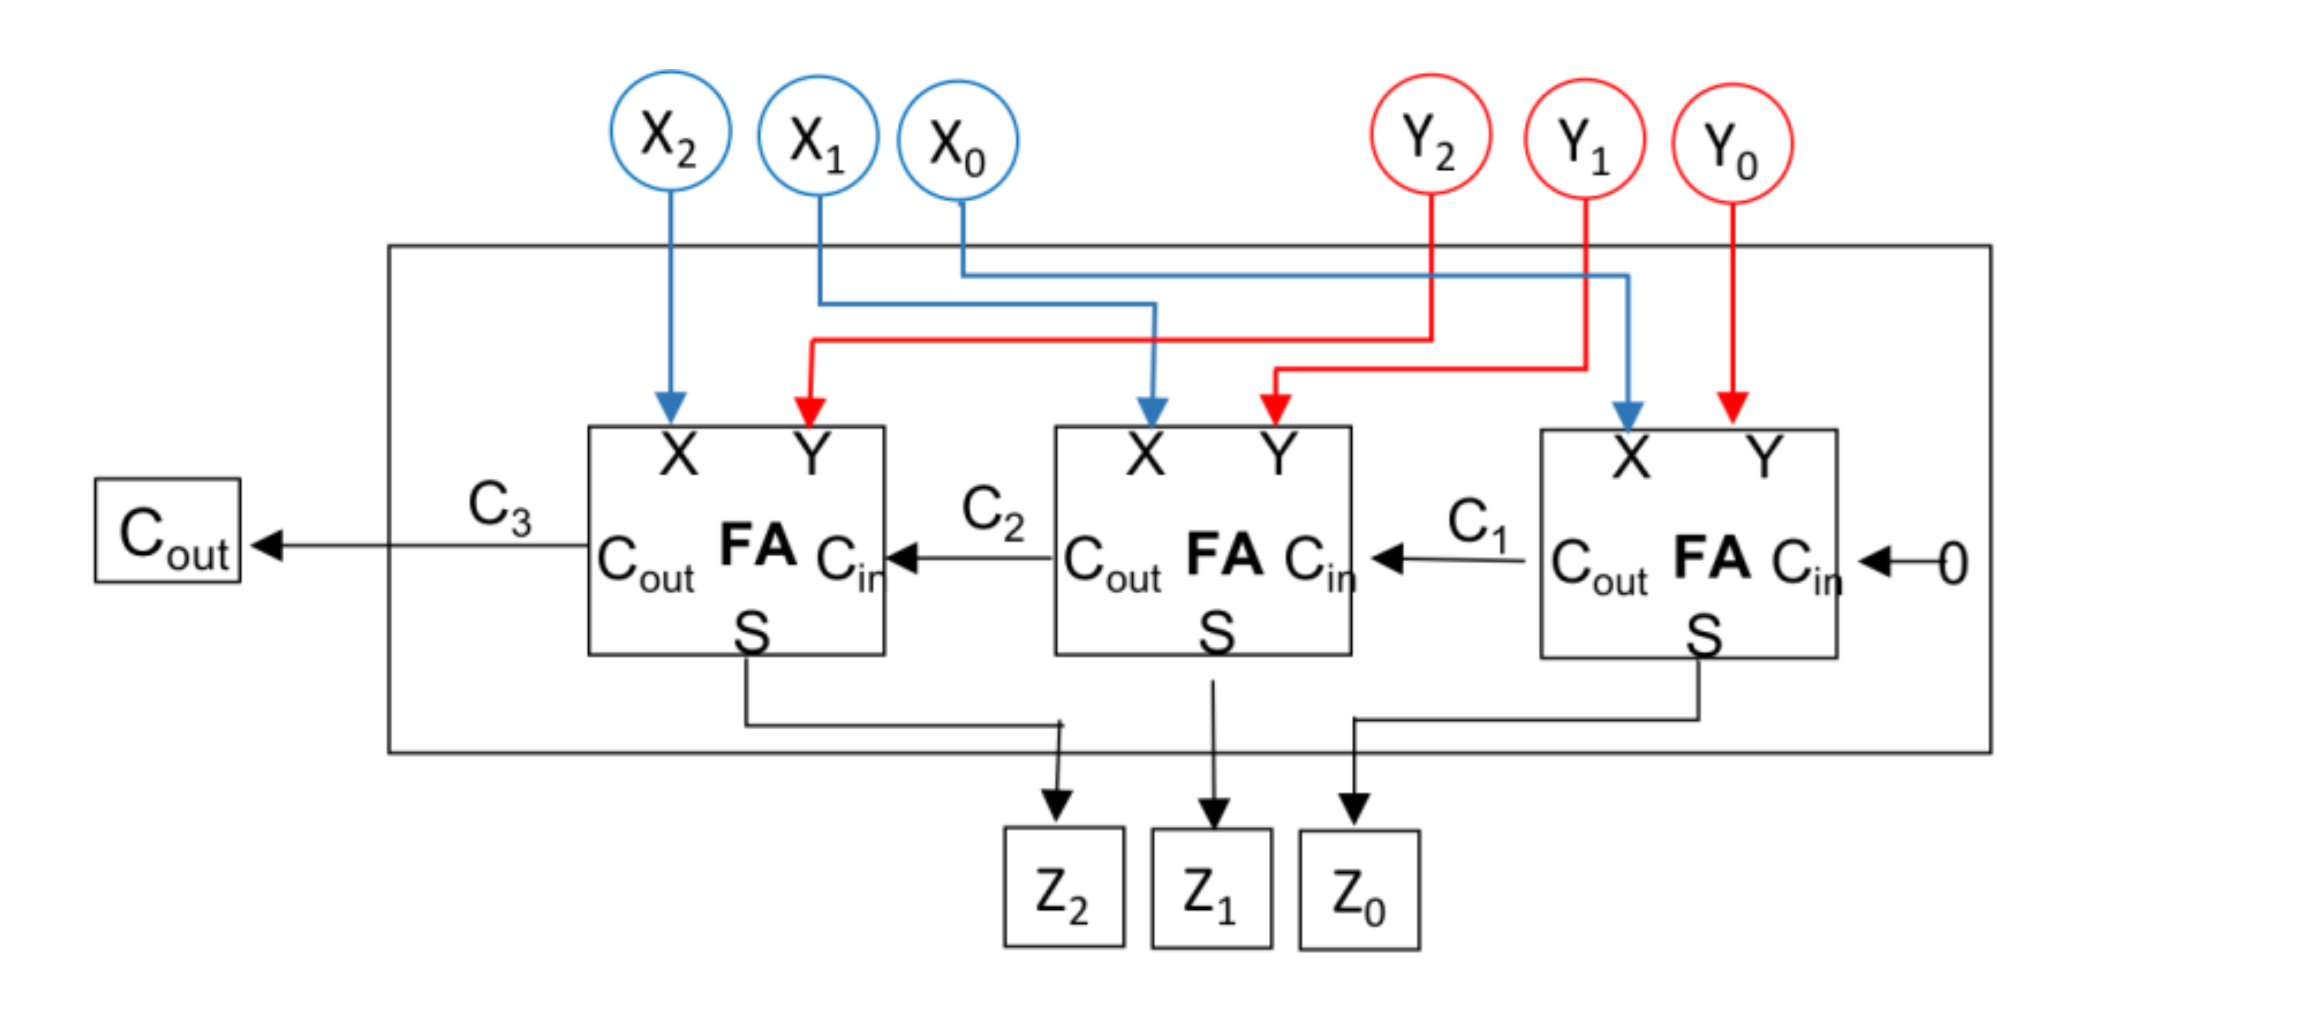
\includegraphics[scale=.60]{examp111}}
		\caption{The 3x3 bit Full Adder Circuit}
	\end{figure}

	The output \textbf{OVERFLOW} bit, which can be used as a signal for the logic
	to indicate a potentially erroneous operation, can be determined quickly by comparing the MSB of Y and
	X. The equation can simply be put as:
	\[
		\mathbf{OVERFLOW} = \closure{X_2}\closure{Y_2}Z_2 + X_{2}Y_{2}\closure{Z_{2}}
	\]

\end{examp}
\begin{examp}
	\vspace{.5mm}
	\textbf{Programmable Array Logic}\\
	For this, the task is to draw a PLA for the equation:
	\[
		F = \closure{C}A + BC
	\]
	\begin{figure}[H]
		\center{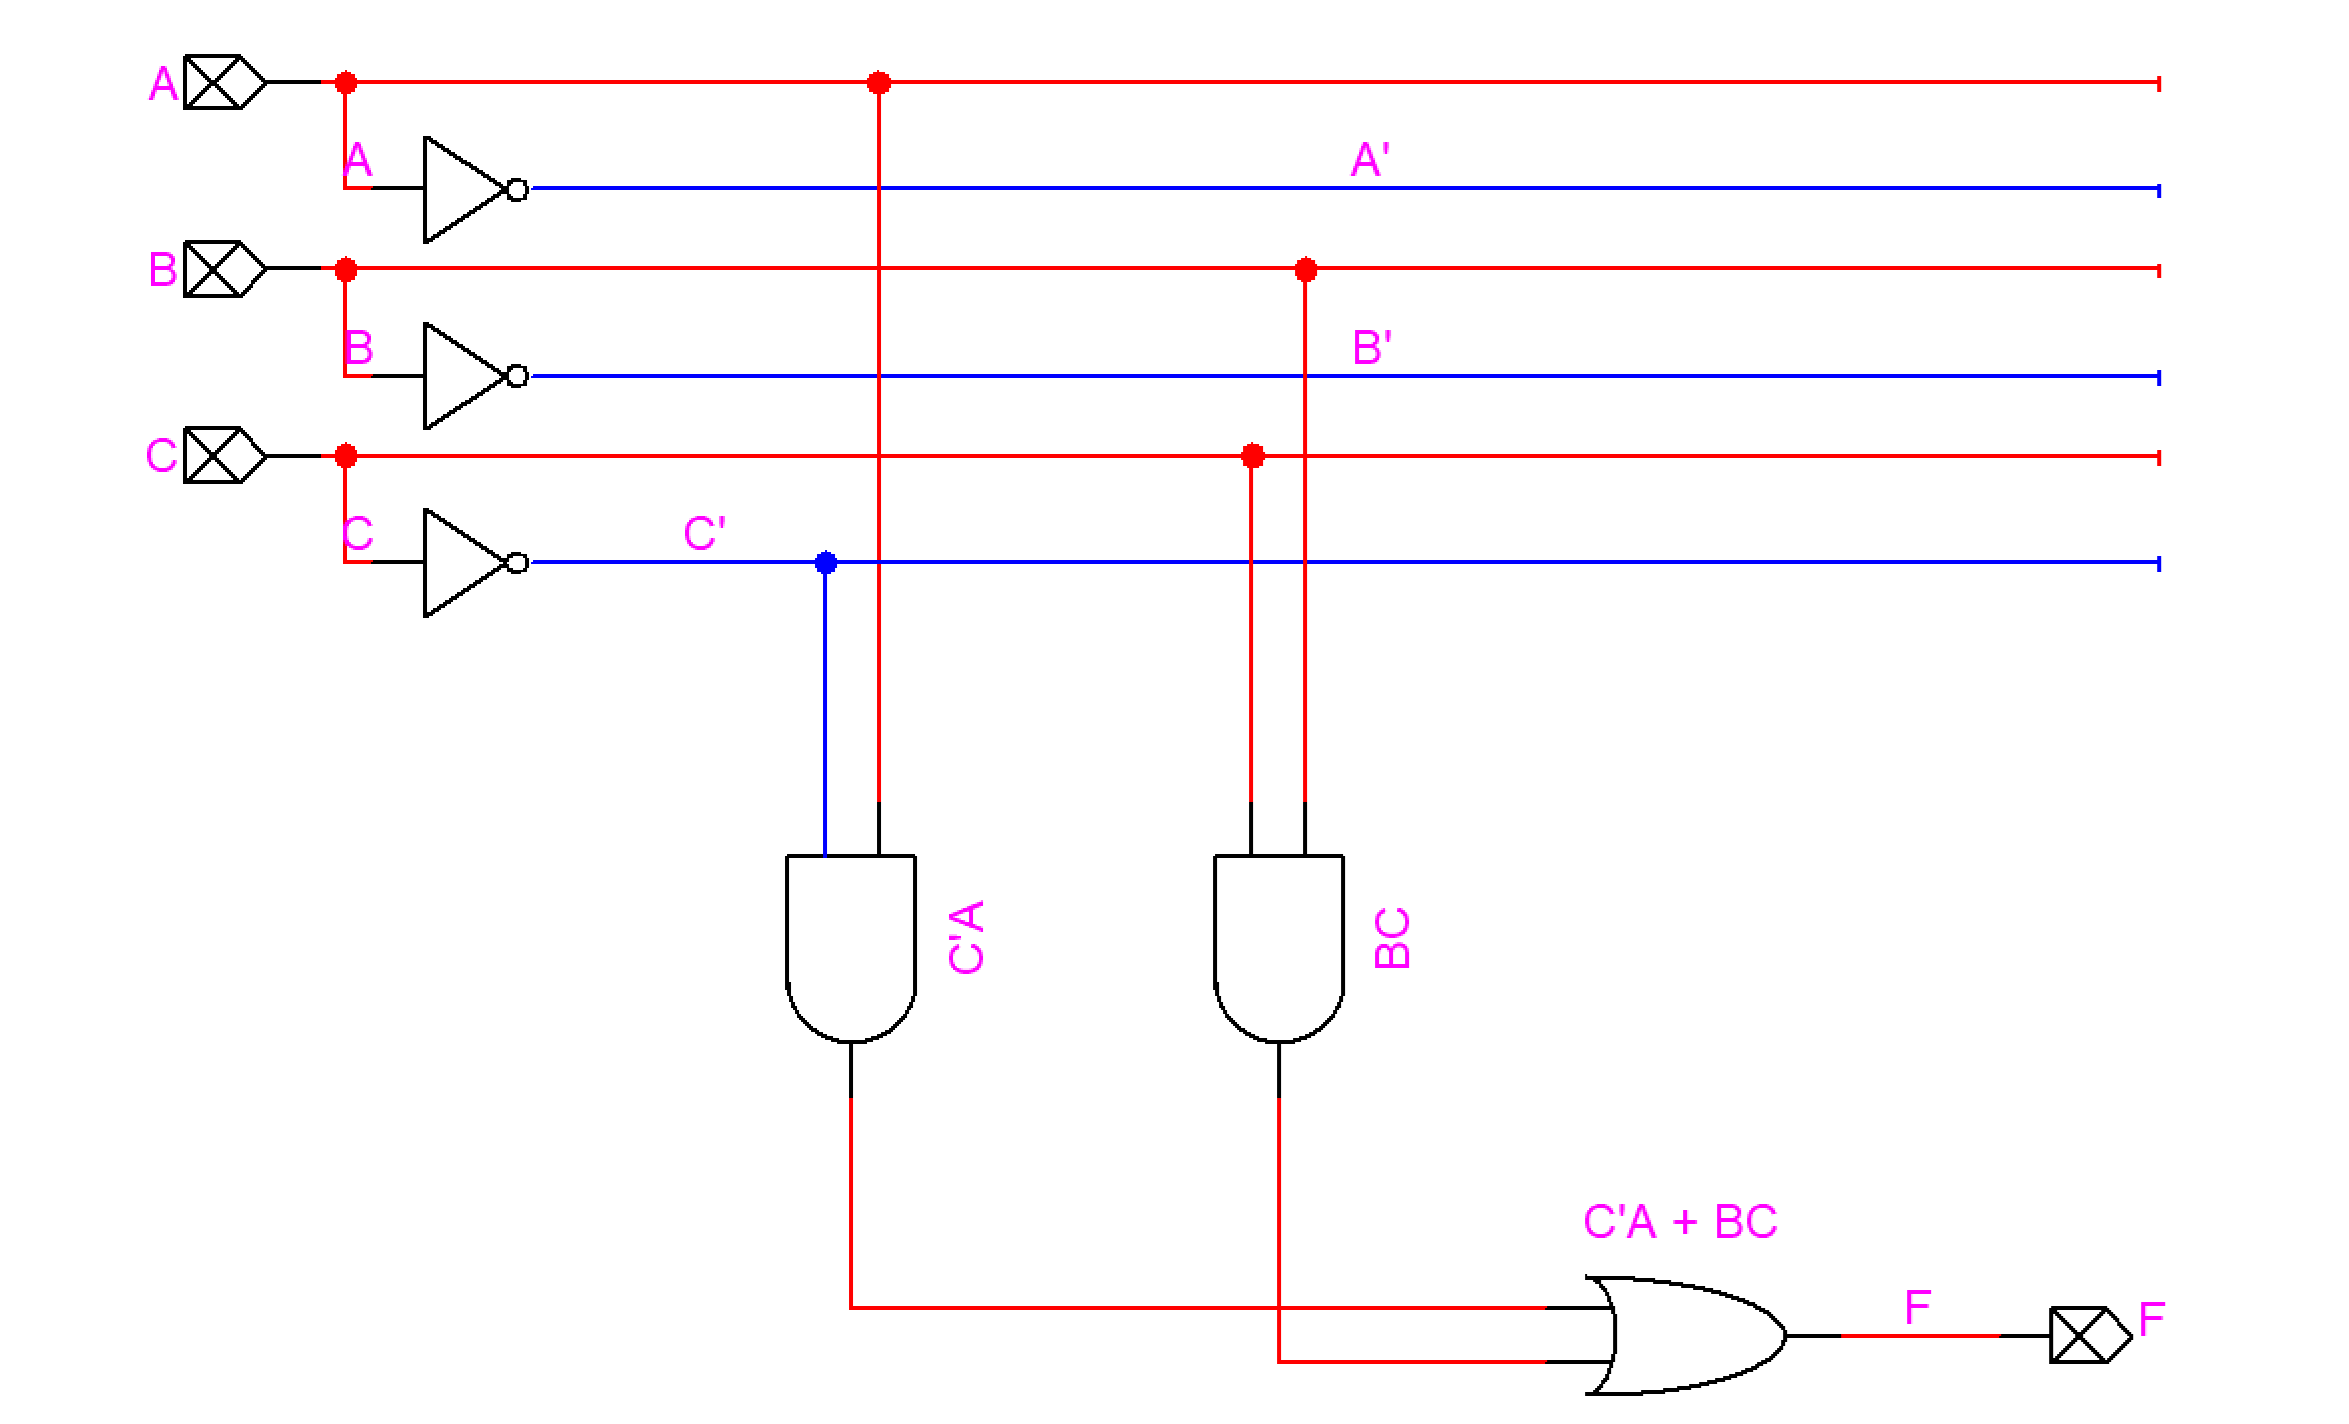
\includegraphics[scale=.50]{examp112}}
		\caption{$F = \closure{C}A + BC$}
	\end{figure}
	This is done similarly to creating combinational logic at the beginning of the
	course. Every wire being drawn out and extended to the combination of AND and
	OR gates is the characteristic of the PLA.
	\vspace{5mm}
\end{examp}
\end{document}
% vim: set tw=80 ts=2 sts=2 sw=2 noai noet:
